\section{Ejercicio V: Comparaci\'on de algoritmos}

Realizamos mediciones sobre instancias aleatorias generadas como describimos en la secci\'on \ref{sec:ej3_exp_instancias}, en particular, instancias chicas para poder ejecutar el algoritmo de backtracking.

Con los datos obtenidos graficamos las distancias obtenidas con cada algoritmo, en cada instancia estudiada, en la figura \ref{fig:ej5_expAleatOp_instancia_distancia}.

\begin{figure}[H]
  \begin{center}
    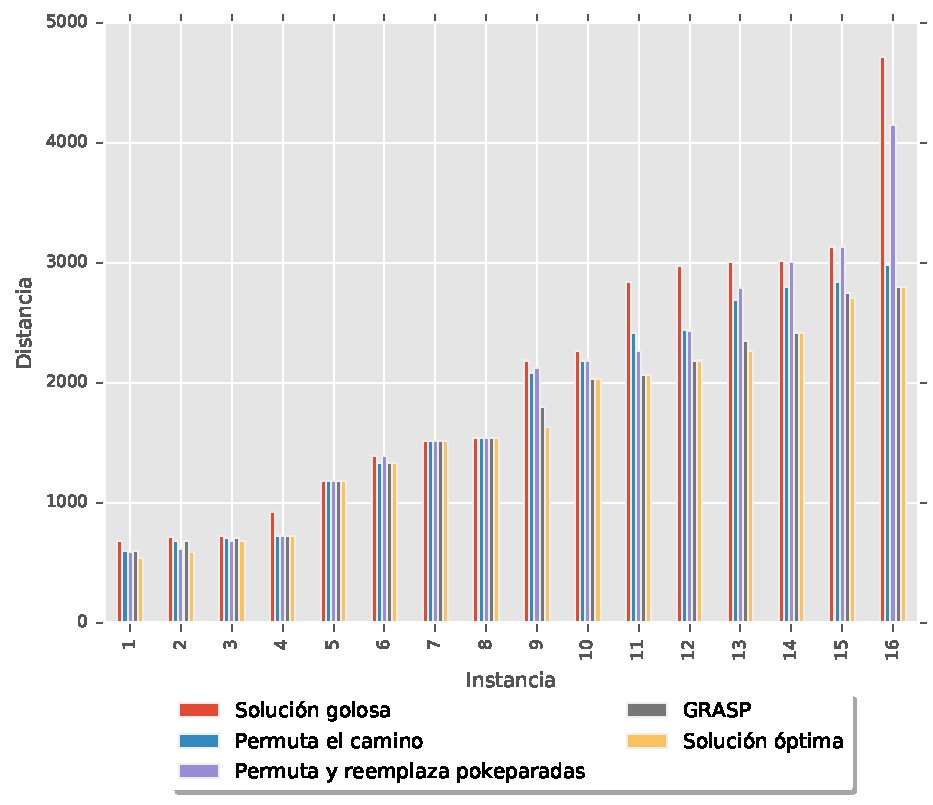
\includegraphics{../experimentacion/ej5/expAleatOp_instancia_distancia.pdf}
    \caption{Distancias computadas para cada una de las instancias analizadas, utilizando instancias aleatorias.}
    \label{fig:ej5_expAleatOp_instancia_distancia}
  \end{center}
\end{figure}

\begin{figure}[H]
  \begin{center}
    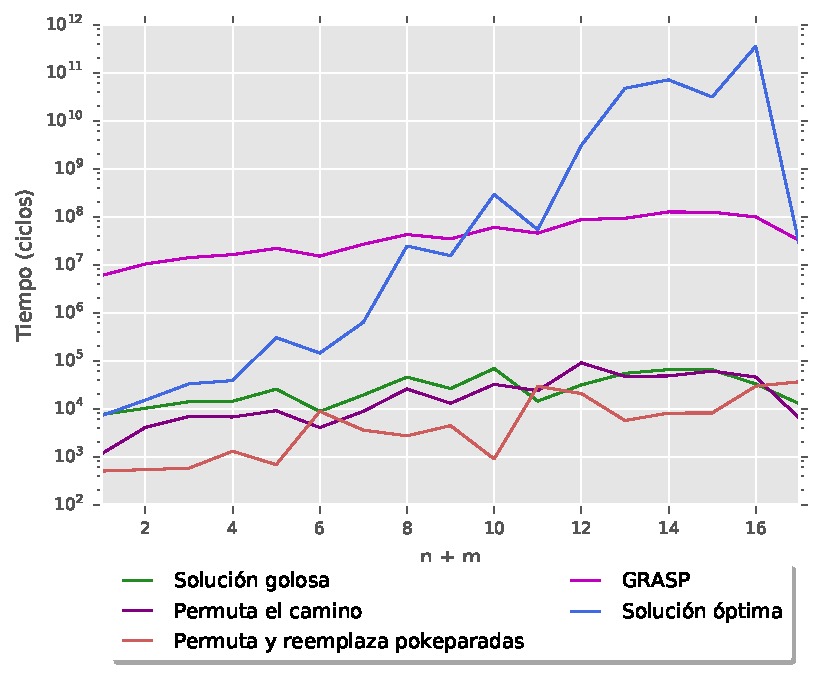
\includegraphics{../experimentacion/ej5/expAleatOp_cantNodos_tiempo.pdf}
    \caption{Tiempo en funci\'on de la cantidad de nodos usando instancias aleatorias.}
    \label{fig:ej5_expAleatOp_cantNodos_tiempo}
  \end{center}
\end{figure}

Exihibimos a continuaci\'on un conjunto de nodos ejemplo del problema, junto con los caminos determinados por los algoritmos desarollados a lo largo de este trabajo:

\begin{figure}[H]
\centering
\begin{minipage}{0.45\textwidth}
\centering
    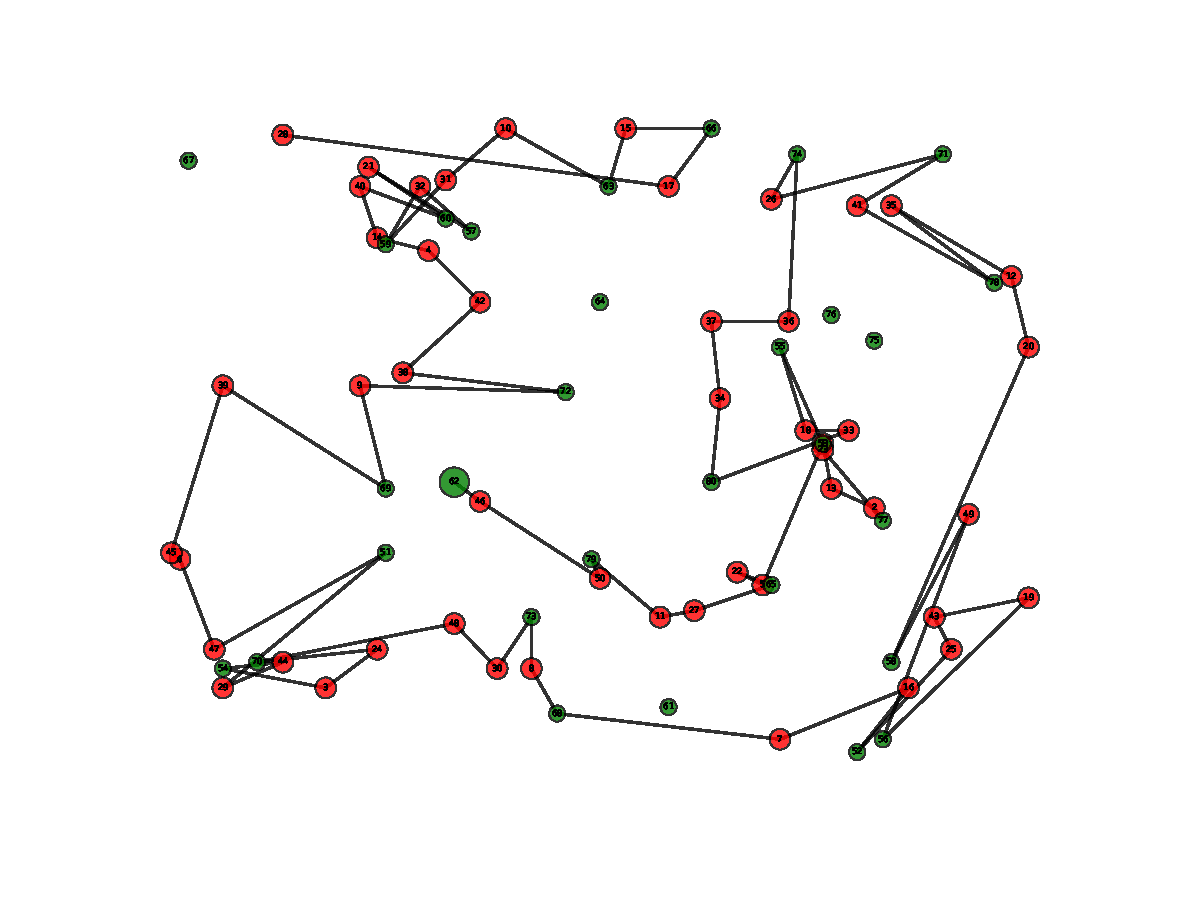
\includegraphics[scale=0.4]{../experimentacion/ej5/ejemplo-salidaSG.pdf}
    \caption{Algoritmo goloso}
    \label{fig:ejemplo-salidaSG}
\end{minipage}
\qquad
\begin{minipage}{0.45\textwidth}
\centering
    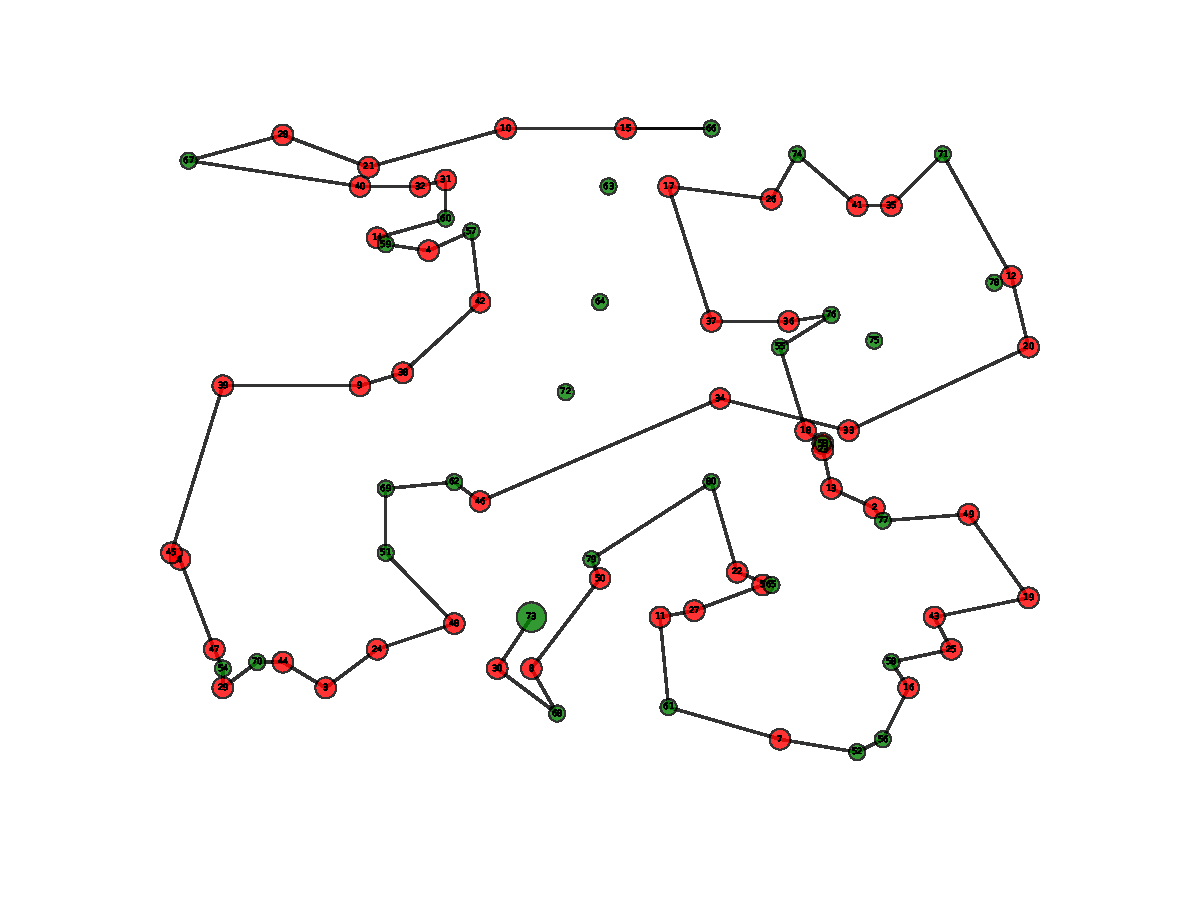
\includegraphics[scale=0.4]{../experimentacion/ej5/ejemplo-salidaGRASP.pdf}
    \caption{GRASP}
    \label{fig:ejemplo-salidaGRASP}
\end{minipage}
\end{figure}

\begin{figure}[H]
\centering
\begin{minipage}{0.45\textwidth}
\centering
    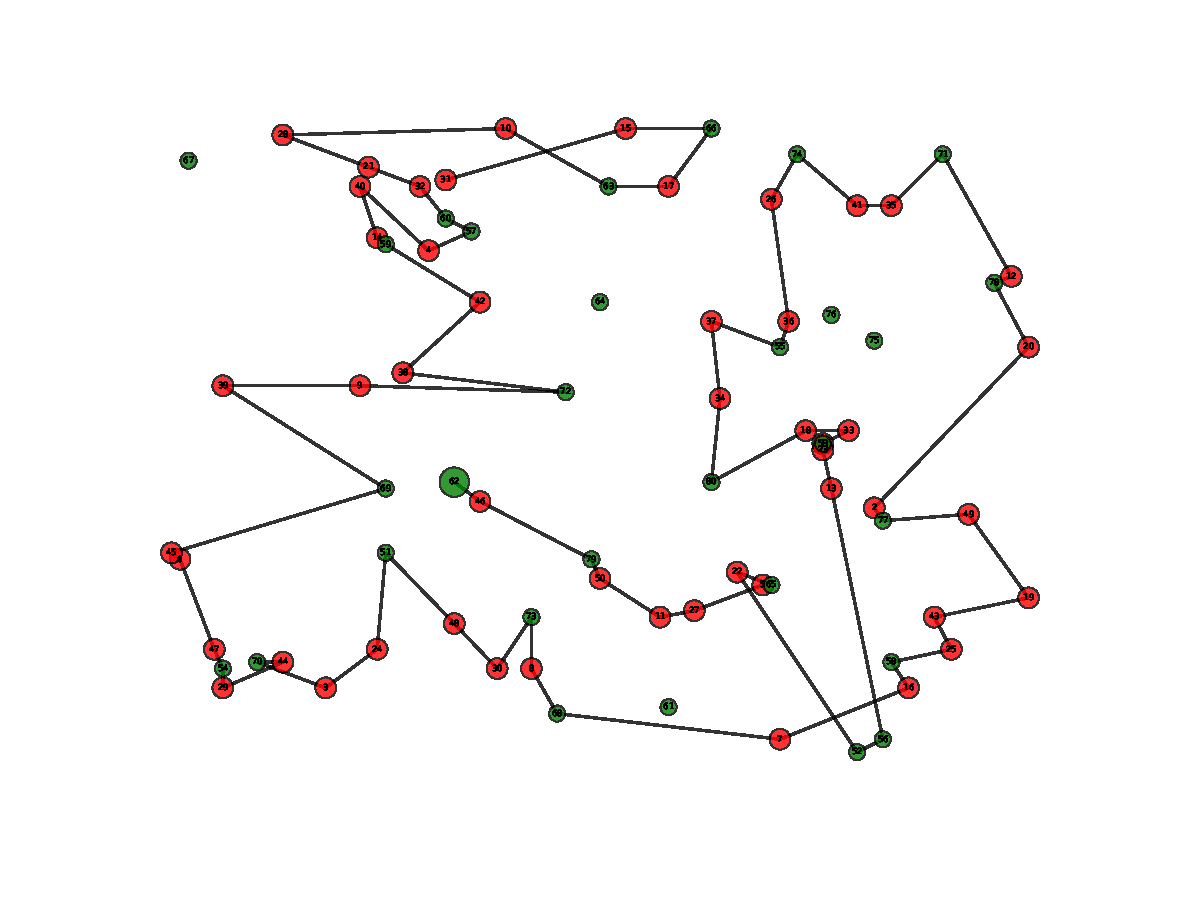
\includegraphics[scale=0.4]{../experimentacion/ej5/ejemplo-salidaBLPC.pdf}
    \caption{B\'usqueda local permutando el camino}
    \label{fig:ejemplo-salidaBLPC}
\end{minipage}
\qquad
\begin{minipage}{0.45\textwidth}
\centering
    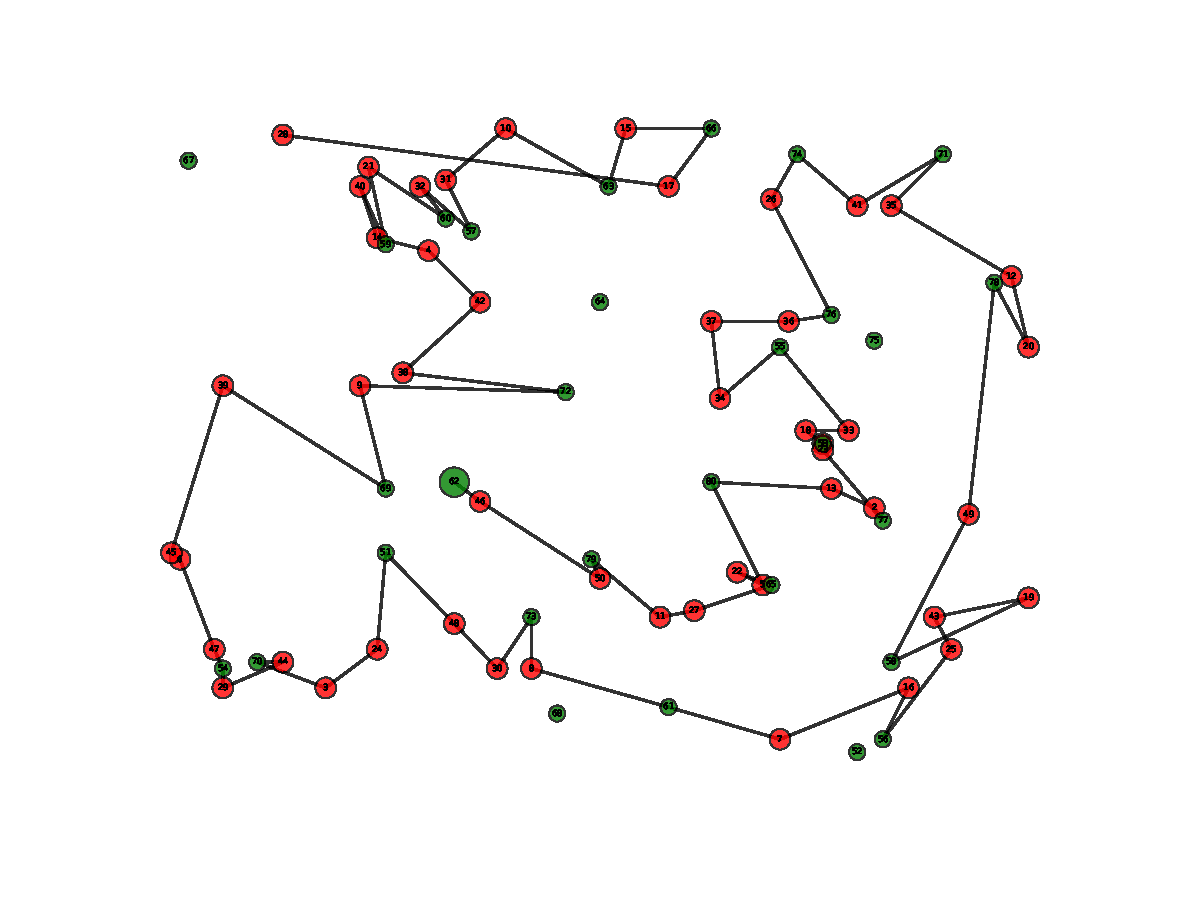
\includegraphics[scale=0.4]{../experimentacion/ej5/ejemplo-salidaBLPYRP.pdf}
    \caption{B\'usqueda local permutando y reemplazando pokeparadas}
    \label{fig:ejemplo-salidaBLPYRP}
\end{minipage}
\end{figure}